\documentclass[color=usenames,dvipsnames]{beamer}\usepackage[]{graphicx}\usepackage[]{color}
% maxwidth is the original width if it is less than linewidth
% otherwise use linewidth (to make sure the graphics do not exceed the margin)
\makeatletter
\def\maxwidth{ %
  \ifdim\Gin@nat@width>\linewidth
    \linewidth
  \else
    \Gin@nat@width
  \fi
}
\makeatother

\definecolor{fgcolor}{rgb}{0.345, 0.345, 0.345}
\newcommand{\hlnum}[1]{\textcolor[rgb]{0.686,0.059,0.569}{#1}}%
\newcommand{\hlstr}[1]{\textcolor[rgb]{0.192,0.494,0.8}{#1}}%
\newcommand{\hlcom}[1]{\textcolor[rgb]{0.678,0.584,0.686}{\textit{#1}}}%
\newcommand{\hlopt}[1]{\textcolor[rgb]{0,0,0}{#1}}%
\newcommand{\hlstd}[1]{\textcolor[rgb]{0.345,0.345,0.345}{#1}}%
\newcommand{\hlkwa}[1]{\textcolor[rgb]{0.161,0.373,0.58}{\textbf{#1}}}%
\newcommand{\hlkwb}[1]{\textcolor[rgb]{0.69,0.353,0.396}{#1}}%
\newcommand{\hlkwc}[1]{\textcolor[rgb]{0.333,0.667,0.333}{#1}}%
\newcommand{\hlkwd}[1]{\textcolor[rgb]{0.737,0.353,0.396}{\textbf{#1}}}%
\let\hlipl\hlkwb

\usepackage{framed}
\makeatletter
\newenvironment{kframe}{%
 \def\at@end@of@kframe{}%
 \ifinner\ifhmode%
  \def\at@end@of@kframe{\end{minipage}}%
  \begin{minipage}{\columnwidth}%
 \fi\fi%
 \def\FrameCommand##1{\hskip\@totalleftmargin \hskip-\fboxsep
 \colorbox{shadecolor}{##1}\hskip-\fboxsep
     % There is no \\@totalrightmargin, so:
     \hskip-\linewidth \hskip-\@totalleftmargin \hskip\columnwidth}%
 \MakeFramed {\advance\hsize-\width
   \@totalleftmargin\z@ \linewidth\hsize
   \@setminipage}}%
 {\par\unskip\endMakeFramed%
 \at@end@of@kframe}
\makeatother

\definecolor{shadecolor}{rgb}{.97, .97, .97}
\definecolor{messagecolor}{rgb}{0, 0, 0}
\definecolor{warningcolor}{rgb}{1, 0, 1}
\definecolor{errorcolor}{rgb}{1, 0, 0}
\newenvironment{knitrout}{}{} % an empty environment to be redefined in TeX

\usepackage{alltt}
%\documentclass[color=usenames,dvipsnames,handout]{beamer}

%\usepackage[roman]{../pres1}
\usepackage[sans]{../pres1}
\usepackage{graphicx}
\usepackage{bm}
\usepackage{array}






\IfFileExists{upquote.sty}{\usepackage{upquote}}{}
\begin{document}

%\fontfamily{lmodern}

\begin{frame}[plain]
  \begin{center}
    {\huge \bf Population Viability Analysis \par}
%    \vspace{0.5cm}
%    { \Large March 6, 2019} \\
    {%\color{blue}
      \rule{\textwidth}{0.1pt}}
    \vfill
    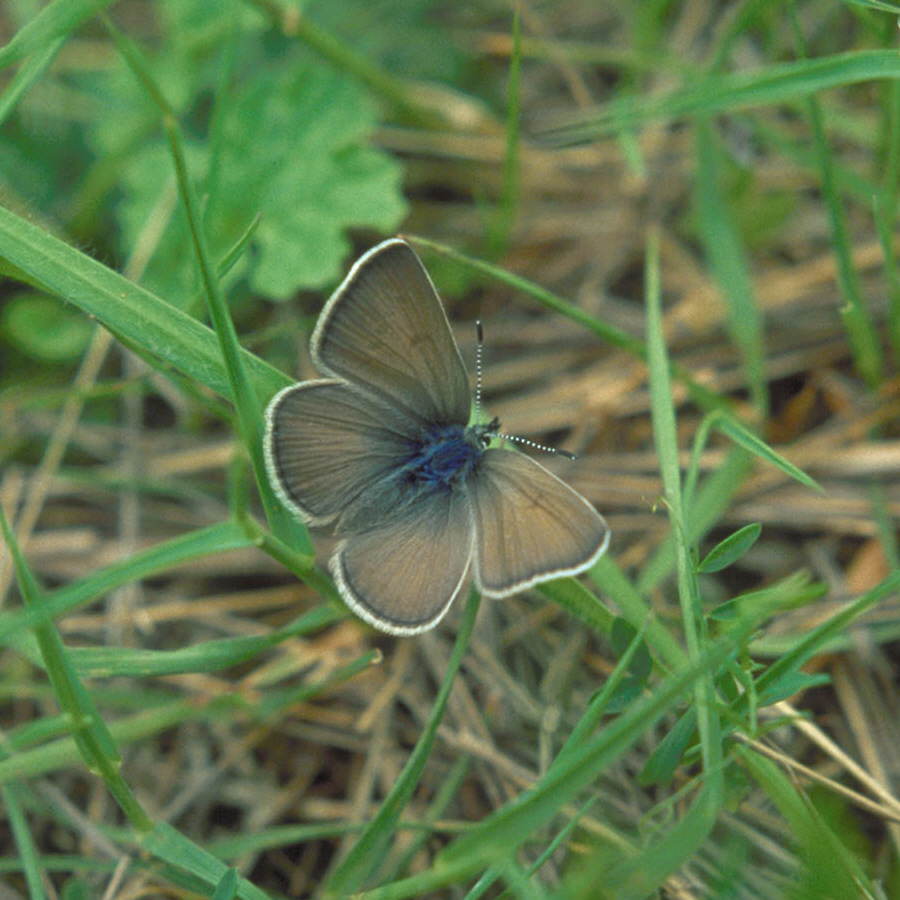
\includegraphics[height=4cm,keepaspectratio]{figs/Fenders_blue} \hfill
%    \hspace{0.5cm}
    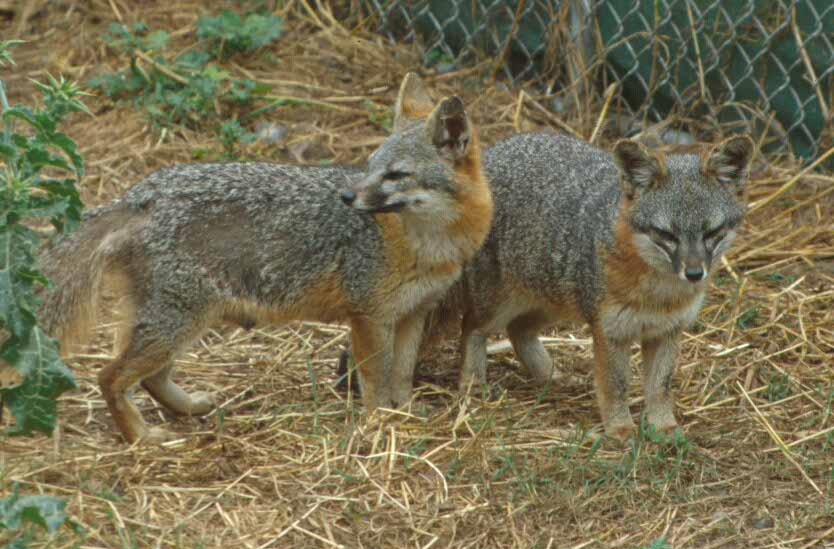
\includegraphics[height=4cm,keepaspectratio]{figs/Urocyon_littoralis}
  \end{center}
\end{frame}




\section{Introduction}





\begin{frame}
  \frametitle{What is PVA?}
  \Large
  {\bf Population Viability Analysis \\}
  \begin{quote}
    The use of quantitative methods to predict the likely future
    status of a population or collection of populations of
    conservation concern.
  \end{quote}
  \small
  \flushright (Morris and Doak 2002) \par
\end{frame}




\begin{frame}
  \frametitle{History}
  First used by Shaffer (1983) to estimate the {\bf minimum viable
    population} size in Yellowstone National Park
  \begin{center}
    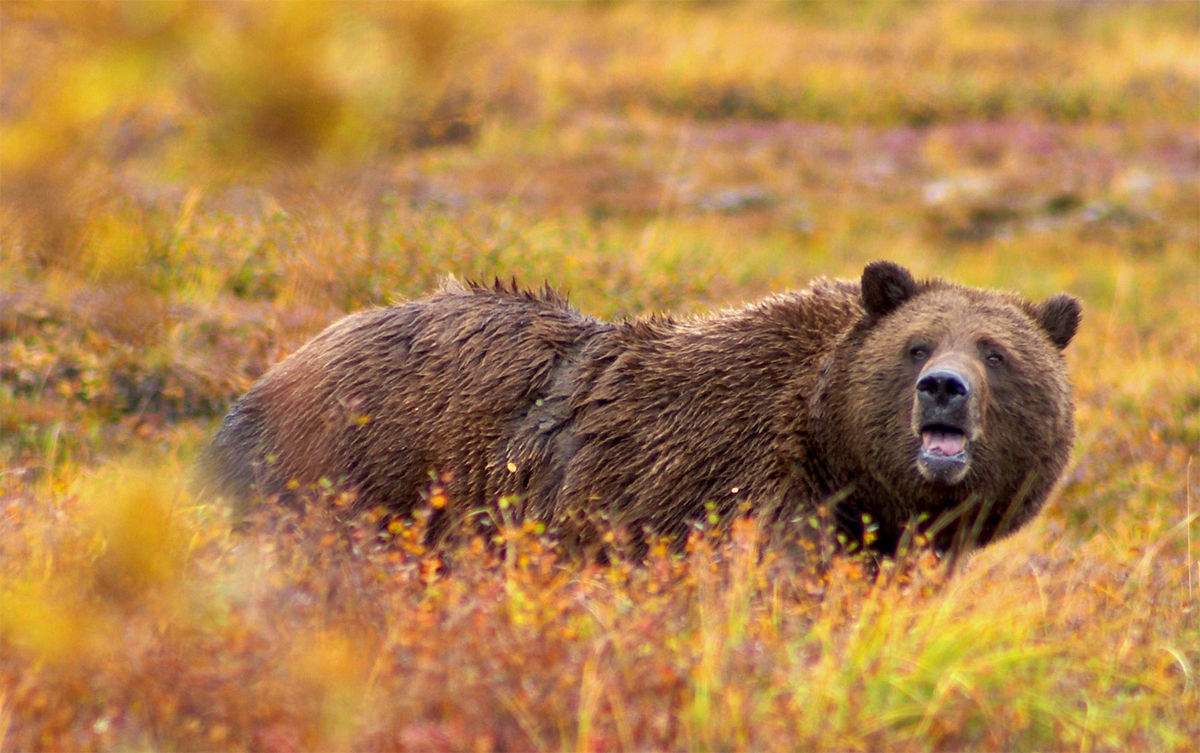
\includegraphics[width=0.7\textwidth]{figs/Grizzly_Denali}
  \end{center}
  \pause
  \centering
  Now routine part of species assessments and recovery plans \\
\end{frame}



% \begin{frame}
%   \frametitle{PVA vs MVP}
%   \large
%   {\bf Population viability analysis\\}
%   Estimating probability of going extinct \par
%   \vspace{1cm}
%   {\bf Minimum viable population \\}
%   Estimating minimum population size \par
% \end{frame}



\section{Uses}




\begin{frame}
  \frametitle{Uses of PVA (from Morris and Doak (2002))}
  \large
%  \setbeamercovered{transparent}
%  \begin{enumerate}[<+-| visible@+->][\bf \color{PineGreen} (1)]
  \begin{enumerate}[\bf (1)]
%    \item<1-| alert@1> Assessing the extinction risk of a single population
%    \item<2-| alert@2> Comparing relative risks of two or more populations
    \item<1-> Assessing the extinction risk of a single population
    \item<2-> Comparing relative risks of two or more populations
    \item<3-> Analyzing and synthesizing monitoring data
    \item<4-| alert@4-> Identifying key life stages or demographic processes as management targets (sensitivity analysis)
    \item<5-> Determining how large a reserve needs to be to achieve a
      desired level of protection from extinction
    \item<6-> Determining how many individuals to release to establish a
      new population
    \item<7-> Setting limits on the harvest or ``take'' from a population
      that are compatible with its continued existence
    \item<8-> Determining how many (and which) populations are needed to
      achieve a desired overall likelihood of species persistence
  \end{enumerate}
\end{frame}




\begin{frame}
  \frametitle{Steps of PVA}
  % \begin{center}
  %   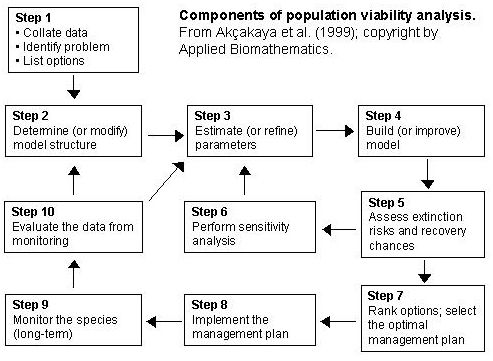
\includegraphics[width=0.9\textwidth]{figs/components}
  % \end{center}
  \large
%  \begin{enumerate}[<+->][\bf (1)]
  \begin{enumerate}[\bf (1)]
    \item Develop objectives
    \item Develop a set of competing models
    \item Design a study to collect necessary data
    \item Fit models to data and select the best model(s)
    \item Use model(s) to identify best management options
    \item Implement management option, monitor the consequences, and refine models
    \item Return to step \color{beamer@blendedblue}{\bf (4)}
  \end{enumerate}
  \vfill
  \centering
%  \uncover<8->{{\bf Very similar to adaptive management} \par}
  \pause
  {\bf Very similar to adaptive management \\}
\end{frame}





\begin{frame}
  \frametitle{Types of PVA}
  \large
%  \begin{enumerate}[<+- | visible@+->][\bf \color{PineGreen} (1)]
  \begin{enumerate}[\bf (1)]
    \item<1-> Count-based PVA
      \begin{itemize}
        \large
        \item All you have is estimates of abundance in each year
        \item This is the cheapest, but least-informative method
      \end{itemize}
    \item<1-> Demographic PVA
      \begin{itemize}
        \large
        \item Requires estimates of vital rates
        \item Useful for identifying key demographic parameters
      \end{itemize}
    \item<1-> Metapopulation viability analysis
      \begin{itemize}
        \large
        \item Useful in reserve design
      \end{itemize}
    \item<1-> Spatially-explicit, individual-based PVA
      \begin{itemize}
        \large
        \item Most realistic, but hardest to parameterize
      \end{itemize}
  \end{enumerate}
  \vfill
  \uncover<2->{\centering \bf All methods require clear definition of time horizon
    and acceptable level of extinction risk \par}
\end{frame}



\begin{frame}
  \frametitle{Products of PVA}
  \begin{center}
    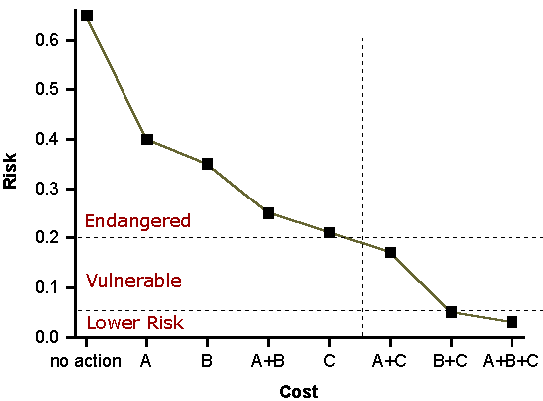
\includegraphics[width=0.9\textwidth]{figs/costben2}
  \end{center}
\end{frame}






\section{Sensitivity Analysis}


\begin{frame}
  \frametitle{Sensitivity analysis}
  A sensitivity analysis seeks to understand the degree to which
  $\lambda$ is sensitive to changes in vital rates.
  \pause
  \vfill
  Usually applied to age- or stage-based population models. \par
  \pause
  \vfill
  The sensitivity of $\lambda$ to a change in a population parameter
  $\theta$ (e.g., survival or fecundity), is:
  \[
%    \text{Sensitivity of}\; \lambda \; \text{to parameter}\; x \;= \frac{\Delta \lambda}{\Delta x}
    \text{sensitivity} = \frac{\Delta \lambda}{\Delta \theta}
  \]
  \pause
  \vfill
  {\bf Sensitivities allow us to make statements such as:} \\
  \begin{quote}
  ``Increasing subadult fecundity by 1 unit increases $\lambda$ by
  0.01, whereas increasing adult fecundity by 1 unit increases $\lambda$ by
  0.02. Therefore, population growth is more sensitive to changes in
  adult fecundity.''
  \end{quote}
\end{frame}



\begin{frame}
  \frametitle{Sensitivity example}
  \centering
  \small
  \begin{tabular}{lccc}
    \hline
    Parameter & $\Delta \theta$ & $\Delta \lambda$ & Sensitivity \\
    \hline
    Fecundity of first age class ($f_1$)  & 0.05 & 0.010 & 0.20 \\ %\pause
    Fecundity of second age class ($f_2$) & 0.05 & 0.003 & 0.06 \\ %\pause
    Survival of first age class ($s_1$)   & 0.05 & 0.040 & 0.80 \\ %\pause
    Survival of second age class ($s_2$)   & 0.05 & 0.030 & 0.60 \\
    \hline
  \end{tabular}
%  \pause
  \vfill
  \normalsize
  \centering Sensitivies don't have to sum to 1 \par
\end{frame}


\begin{frame}
  \frametitle{Elasticity}
  A problem with sensitivities is that it is hard to compare values
  for parameters on different scales, such as survival and
  fecundity. For this reason, it is usually better to report
  ``elasticities'' instead. \\
  \pause
  \vfill
  {\bf Elasticity}: the proportional change in $\lambda$ caused by
  proportional changes in vital rates. \\
  \pause
  \vfill
   Easier interpretation because: %\\
   \begin{itemize}
     \item Standardized units
     \item Values sum to 1
   \end{itemize}
   \pause
   \vfill
   {\bf Examples}
  \begin{itemize}
    \item[] ``A 1\% increase in $f_1$ increases $\lambda$ by 0.01\%.''
    \item[] ``A 1\% increase in $s_1$ increases $\lambda$ by 0.05\%.''
  \end{itemize}

\end{frame}


\begin{frame}[fragile]
  \frametitle{R code for sensitivity analysis}
Suppose we have the following stage-structured projection matrix:
\begin{knitrout}\scriptsize
\definecolor{shadecolor}{rgb}{0.969, 0.969, 0.969}\color{fgcolor}\begin{kframe}
\begin{alltt}
\hlstd{A} \hlkwb{<-} \hlkwd{matrix}\hlstd{(}\hlkwd{c}\hlstd{(}
    \hlnum{0.2}\hlstd{,} \hlnum{0.8}\hlstd{,} \hlnum{1.0}\hlstd{,} \hlnum{0.9}\hlstd{,}
    \hlnum{0.4}\hlstd{,} \hlnum{0.0}\hlstd{,} \hlnum{0.0}\hlstd{,} \hlnum{0.0}\hlstd{,}
    \hlnum{0.0}\hlstd{,} \hlnum{0.6}\hlstd{,} \hlnum{0.0}\hlstd{,} \hlnum{0.0}\hlstd{,}
    \hlnum{0.0}\hlstd{,} \hlnum{0.0}\hlstd{,} \hlnum{0.8}\hlstd{,} \hlnum{0.5}\hlstd{),} \hlkwc{nrow}\hlstd{=}\hlnum{4}\hlstd{,} \hlkwc{byrow}\hlstd{=}\hlnum{TRUE}\hlstd{)}
\end{alltt}
\end{kframe}
\end{knitrout}

We can use eigenanalysis to compute $\lambda$, stable age
distribution, and reproductive value.

\begin{knitrout}\scriptsize
\definecolor{shadecolor}{rgb}{0.969, 0.969, 0.969}\color{fgcolor}\begin{kframe}
\begin{alltt}
\hlstd{eA} \hlkwb{<-} \hlkwd{eigen}\hlstd{(A)}
\hlstd{lam} \hlkwb{<-} \hlkwd{Re}\hlstd{(eA}\hlopt{$}\hlstd{values[}\hlnum{1}\hlstd{])}
\hlstd{lam}                              \hlcom{## Asymtotic growth rate}
\end{alltt}
\begin{verbatim}
## [1] 1.034908
\end{verbatim}
\begin{alltt}
\hlstd{w} \hlkwb{<-} \hlkwd{Re}\hlstd{(eA}\hlopt{$}\hlstd{vectors[,}\hlnum{1}\hlstd{])}
\hlstd{w} \hlkwb{<-} \hlstd{w}\hlopt{/}\hlkwd{sum}\hlstd{(w)}                    \hlcom{## Stable age distribution}

\hlstd{v} \hlkwb{<-} \hlkwd{Re}\hlstd{(}\hlkwd{eigen}\hlstd{(}\hlkwd{t}\hlstd{(A))}\hlopt{$}\hlstd{vectors[,}\hlnum{1}\hlstd{])} \hlcom{## Reproductive value}
\end{alltt}
\end{kframe}
\end{knitrout}

\end{frame}


\begin{frame}[fragile]
  \frametitle{R code for sensitivity analysis}
  The sensitivities are given by $z_{ij}=\frac{v_i w_j}{{\bf v}{\bf w}}$
\begin{knitrout}\scriptsize
\definecolor{shadecolor}{rgb}{0.969, 0.969, 0.969}\color{fgcolor}\begin{kframe}
\begin{alltt}
\hlstd{z} \hlkwb{<-} \hlkwd{outer}\hlstd{(v,w)}\hlopt{/}\hlkwd{c}\hlstd{(v}\hlopt\hlstd{w)}
\hlstd{z} \hlcom{## Sensitivites}
\end{alltt}
\begin{verbatim}
##           [,1]      [,2]       [,3]      [,4]
## [1,] 0.3473925 0.1342698 0.07784447 0.1164229
## [2,] 0.7251023 0.2802575 0.16248251 0.2430061
## [3,] 0.7875009 0.3043751 0.17646493 0.2639179
## [4,] 0.5844985 0.2259131 0.13097572 0.1958851
\end{verbatim}
\end{kframe}
\end{knitrout}
\pause
\vfill
The elasticities are given by $e_{ij}=\frac{a_{ij}z_{ij}}{\lambda}$
\begin{knitrout}\scriptsize
\definecolor{shadecolor}{rgb}{0.969, 0.969, 0.969}\color{fgcolor}\begin{kframe}
\begin{alltt}
\hlstd{e} \hlkwb{<-} \hlstd{A}\hlopt{*}\hlstd{z}\hlopt{/}\hlstd{lam}
\hlstd{e}  \hlcom{## Elasticities}
\end{alltt}
\begin{verbatim}
##            [,1]      [,2]      [,3]       [,4]
## [1,] 0.06713492 0.1037926 0.0752187 0.10124623
## [2,] 0.28025755 0.0000000 0.0000000 0.00000000
## [3,] 0.00000000 0.1764649 0.0000000 0.00000000
## [4,] 0.00000000 0.0000000 0.1012462 0.09463883
\end{verbatim}
\end{kframe}
\end{knitrout}

\end{frame}



\begin{frame}
  \frametitle{Sensitivity and elasticity}
 {\bf Take-home points} \\
 \vfill
  Sensitivity measures the change in $\lambda$ given an absolute
  change in a parameter. \\
  \vfill
  Elasticity measures the proportional change in $\lambda$ given a
  proportional change in a parameter.
\end{frame}




\section{Summary}



\begin{frame}
  \frametitle{Problems with PVA}
  \large
  Most PVA's are {\it ``essentially games played with
    guesses.''} (Caughley, G. 1994. Conservation Biology) \par
  \pause
  \vspace{0.5cm}
  Many PVA's don't include multiple models corresponding to different
  hypotheses. \par
  \pause
  \vspace{0.5cm}
  {Some software encourages this. \\}
\end{frame}




\begin{frame}
  \frametitle{Summary}
  \large
  {\bf Final thoughts}
  \begin{itemize}[<+->]
    \item People often say that PVA's require too much data.
    \item[]
    \item But what is the alternative?
    \item[]
    \item When data are limited (and they always are), you must
      decrease the time horizon and acknowledge uncertainty in decision process. 
  \end{itemize}
\end{frame}


\begin{comment}
\begin{knitrout}
\definecolor{shadecolor}{rgb}{0.969, 0.969, 0.969}\color{fgcolor}\begin{kframe}
\begin{alltt}
\hlstd{A} \hlkwb{<-} \hlkwd{matrix}\hlstd{(}\hlkwd{c}\hlstd{(}
    \hlnum{0.2}\hlstd{,} \hlnum{0.8}\hlstd{,} \hlnum{1.0}\hlstd{,} \hlnum{0.9}\hlstd{,}
    \hlnum{0.4}\hlstd{,} \hlnum{0.0}\hlstd{,} \hlnum{0.0}\hlstd{,} \hlnum{0.0}\hlstd{,}
    \hlnum{0.0}\hlstd{,} \hlnum{0.6}\hlstd{,} \hlnum{0.0}\hlstd{,} \hlnum{0.0}\hlstd{,}
    \hlnum{0.0}\hlstd{,} \hlnum{0.0}\hlstd{,} \hlnum{0.8}\hlstd{,} \hlnum{0.5}\hlstd{),} \hlkwc{nrow}\hlstd{=}\hlnum{4}\hlstd{,} \hlkwc{byrow}\hlstd{=}\hlnum{TRUE}\hlstd{)}
\hlstd{eA} \hlkwb{<-} \hlkwd{eigen}\hlstd{(A)}
\hlstd{eA}
\end{alltt}
\begin{verbatim}
## eigen() decomposition
## $values
## [1]  1.0349085+0.0000000i  0.0164566+0.3720685i  0.0164566-0.3720685i
## [4] -0.3678217+0.0000000i
## 
## $vectors
##               [,1]                  [,2]                  [,3]          [,4]
## [1,] -0.8730660+0i  0.2292637-0.2111293i  0.2292637+0.2111293i  0.3534730+0i
## [2,] -0.3374467+0i -0.2156555-0.2560132i -0.2156555+0.2560132i -0.3843961+0i
## [3,] -0.1956386+0i -0.4273941+0.3288637i -0.4273941-0.3288637i  0.6270365+0i
## [4,] -0.2925937+0i  0.7071036+0.0000000i  0.7071036+0.0000000i -0.5780326+0i
\end{verbatim}
\begin{alltt}
\hlstd{lam} \hlkwb{<-} \hlkwd{Re}\hlstd{(eA}\hlopt{$}\hlstd{values[}\hlnum{1}\hlstd{])}
\hlstd{lam}
\end{alltt}
\begin{verbatim}
## [1] 1.034908
\end{verbatim}
\begin{alltt}
\hlstd{w} \hlkwb{<-} \hlkwd{Re}\hlstd{(eA}\hlopt{$}\hlstd{vectors[,}\hlnum{1}\hlstd{])}
\hlstd{w}
\end{alltt}
\begin{verbatim}
## [1] -0.8730660 -0.3374467 -0.1956386 -0.2925937
\end{verbatim}
\begin{alltt}
\hlstd{v} \hlkwb{<-} \hlkwd{Re}\hlstd{(}\hlkwd{eigen}\hlstd{(}\hlkwd{t}\hlstd{(A))}\hlopt{$}\hlstd{vectors[,}\hlnum{1}\hlstd{])}
\hlstd{v}
\end{alltt}
\begin{verbatim}
## [1] 0.2739325 0.5717713 0.6209750 0.4608998
\end{verbatim}
\begin{alltt}
\hlstd{sen} \hlkwb{<-} \hlkwd{outer}\hlstd{(v,w)}\hlopt{/}\hlkwd{c}\hlstd{(v}\hlopt\hlstd{w)}
\hlstd{sen}
\end{alltt}
\begin{verbatim}
##           [,1]      [,2]       [,3]      [,4]
## [1,] 0.3473925 0.1342698 0.07784447 0.1164229
## [2,] 0.7251023 0.2802575 0.16248251 0.2430061
## [3,] 0.7875009 0.3043751 0.17646493 0.2639179
## [4,] 0.5844985 0.2259131 0.13097572 0.1958851
\end{verbatim}
\begin{alltt}
\hlstd{el} \hlkwb{<-} \hlstd{A}\hlopt{*}\hlstd{sen}\hlopt{/}\hlstd{lam}
\hlstd{el}
\end{alltt}
\begin{verbatim}
##            [,1]      [,2]      [,3]       [,4]
## [1,] 0.06713492 0.1037926 0.0752187 0.10124623
## [2,] 0.28025755 0.0000000 0.0000000 0.00000000
## [3,] 0.00000000 0.1764649 0.0000000 0.00000000
## [4,] 0.00000000 0.0000000 0.1012462 0.09463883
\end{verbatim}
\begin{alltt}
\hlstd{A2} \hlkwb{<-} \hlstd{A}
\hlstd{A2[}\hlnum{1}\hlstd{,}\hlnum{1}\hlstd{]} \hlkwb{<-} \hlstd{A[}\hlnum{1}\hlstd{,}\hlnum{1}\hlstd{]}\hlopt{+}\hlnum{0.1}
\hlstd{lam2} \hlkwb{<-} \hlkwd{Re}\hlstd{(}\hlkwd{eigen}\hlstd{(A2)}\hlopt{$}\hlstd{val[}\hlnum{1}\hlstd{])}

\hlstd{A3} \hlkwb{<-} \hlstd{A}
\hlstd{A3[}\hlnum{1}\hlstd{,}\hlnum{2}\hlstd{]} \hlkwb{<-} \hlstd{A[}\hlnum{1}\hlstd{,}\hlnum{2}\hlstd{]}\hlopt{+}\hlnum{0.1}
\hlstd{lam3} \hlkwb{<-} \hlkwd{Re}\hlstd{(}\hlkwd{eigen}\hlstd{(A3)}\hlopt{$}\hlstd{val[}\hlnum{1}\hlstd{])}

\hlstd{(lam2}\hlopt{-}\hlstd{lam)}\hlopt{/}\hlnum{0.1}
\end{alltt}
\begin{verbatim}
## [1] 0.3641666
\end{verbatim}
\begin{alltt}
\hlstd{(lam3}\hlopt{-}\hlstd{lam)}\hlopt{/}\hlnum{0.1}
\end{alltt}
\begin{verbatim}
## [1] 0.1349474
\end{verbatim}
\end{kframe}
\end{knitrout}

\end{comment}



\end{document}


